%%%%%%%%%%%%%%%%%%%%%%%%%%%%%%%%%%%%%%%%%%%%%%%%

% Specify the command that you want into the header of the
% index.md file

%%%%%%%%%%%%%%%%%%%%%%%%%%%%%%%%%%%%%%%%%%%%%%%%

% Options for packages loaded elsewhere
\PassOptionsToPackage{unicode}{hyperref}
\PassOptionsToPackage{hyphens}{url}
\PassOptionsToPackage{dvipsnames,svgnames*,x11names*}{xcolor}
%
\documentclass[
  12pt,
  oneside]{report}
%%\usepackage{lmodern}
%
% Set line spacing
\usepackage{setspace}
\setstretch{1.5}

\usepackage{amssymb,amsmath}
\usepackage{ifxetex,ifluatex}
\ifnum 0\ifxetex 1\fi\ifluatex 1\fi=0 % if pdftex
  \usepackage[T1]{fontenc}
  \usepackage[utf8]{inputenc}
  \usepackage{textcomp} % provide euro and other symbols
\else % if luatex or xetex
  \usepackage{unicode-math}
  \defaultfontfeatures{Scale=MatchLowercase}
  \defaultfontfeatures[\rmfamily]{Ligatures=TeX,Scale=1}
\fi
% Use upquote if available, for straight quotes in verbatim environments
\IfFileExists{upquote.sty}{\usepackage{upquote}}{}
\IfFileExists{microtype.sty}{% use microtype if available
  \usepackage[]{microtype}
  \UseMicrotypeSet[protrusion]{basicmath} % disable protrusion for tt fonts
}{}
\makeatletter
\@ifundefined{KOMAClassName}{% if non-KOMA class
  \IfFileExists{parskip.sty}{%
    \usepackage{parskip}
  }{% else
    \setlength{\parindent}{0pt}
    \setlength{\parskip}{6pt plus 2pt minus 1pt}}
}{% if KOMA class
  \KOMAoptions{parskip=half}}
\makeatother
\usepackage{xcolor}
\IfFileExists{xurl.sty}{\usepackage{xurl}}{} % add URL line breaks if available
\IfFileExists{bookmark.sty}{\usepackage{bookmark}}{\usepackage{hyperref}}
\hypersetup{
  pdfauthor={François Leroy, PhD student at CZU},
  colorlinks=true,
  linkcolor=Maroon,
  filecolor=Maroon,
  citecolor=Blue,
  urlcolor=Blue,
  pdfcreator={LaTeX via pandoc}}
\urlstyle{same} % disable monospaced font for URLs

%% Package geometry
\usepackage[left = 2cm,right = 2cm,top = 2cm,bottom = 2cm]{geometry}
\usepackage{pdflscape}


\usepackage{color}
\usepackage{fancyvrb}
\newcommand{\VerbBar}{|}
\newcommand{\VERB}{\Verb[commandchars=\\\{\}]}
\DefineVerbatimEnvironment{Highlighting}{Verbatim}{commandchars=\\\{\}}
% Add ',fontsize=\small' for more characters per line
\usepackage{framed}
\definecolor{shadecolor}{RGB}{248,248,248}
\newenvironment{Shaded}{\begin{snugshade}}{\end{snugshade}}
\newcommand{\AlertTok}[1]{\textcolor[rgb]{0.94,0.16,0.16}{#1}}
\newcommand{\AnnotationTok}[1]{\textcolor[rgb]{0.56,0.35,0.01}{\textbf{\textit{#1}}}}
\newcommand{\AttributeTok}[1]{\textcolor[rgb]{0.77,0.63,0.00}{#1}}
\newcommand{\BaseNTok}[1]{\textcolor[rgb]{0.00,0.00,0.81}{#1}}
\newcommand{\BuiltInTok}[1]{#1}
\newcommand{\CharTok}[1]{\textcolor[rgb]{0.31,0.60,0.02}{#1}}
\newcommand{\CommentTok}[1]{\textcolor[rgb]{0.56,0.35,0.01}{\textit{#1}}}
\newcommand{\CommentVarTok}[1]{\textcolor[rgb]{0.56,0.35,0.01}{\textbf{\textit{#1}}}}
\newcommand{\ConstantTok}[1]{\textcolor[rgb]{0.00,0.00,0.00}{#1}}
\newcommand{\ControlFlowTok}[1]{\textcolor[rgb]{0.13,0.29,0.53}{\textbf{#1}}}
\newcommand{\DataTypeTok}[1]{\textcolor[rgb]{0.13,0.29,0.53}{#1}}
\newcommand{\DecValTok}[1]{\textcolor[rgb]{0.00,0.00,0.81}{#1}}
\newcommand{\DocumentationTok}[1]{\textcolor[rgb]{0.56,0.35,0.01}{\textbf{\textit{#1}}}}
\newcommand{\ErrorTok}[1]{\textcolor[rgb]{0.64,0.00,0.00}{\textbf{#1}}}
\newcommand{\ExtensionTok}[1]{#1}
\newcommand{\FloatTok}[1]{\textcolor[rgb]{0.00,0.00,0.81}{#1}}
\newcommand{\FunctionTok}[1]{\textcolor[rgb]{0.00,0.00,0.00}{#1}}
\newcommand{\ImportTok}[1]{#1}
\newcommand{\InformationTok}[1]{\textcolor[rgb]{0.56,0.35,0.01}{\textbf{\textit{#1}}}}
\newcommand{\KeywordTok}[1]{\textcolor[rgb]{0.13,0.29,0.53}{\textbf{#1}}}
\newcommand{\NormalTok}[1]{#1}
\newcommand{\OperatorTok}[1]{\textcolor[rgb]{0.81,0.36,0.00}{\textbf{#1}}}
\newcommand{\OtherTok}[1]{\textcolor[rgb]{0.56,0.35,0.01}{#1}}
\newcommand{\PreprocessorTok}[1]{\textcolor[rgb]{0.56,0.35,0.01}{\textit{#1}}}
\newcommand{\RegionMarkerTok}[1]{#1}
\newcommand{\SpecialCharTok}[1]{\textcolor[rgb]{0.00,0.00,0.00}{#1}}
\newcommand{\SpecialStringTok}[1]{\textcolor[rgb]{0.31,0.60,0.02}{#1}}
\newcommand{\StringTok}[1]{\textcolor[rgb]{0.31,0.60,0.02}{#1}}
\newcommand{\VariableTok}[1]{\textcolor[rgb]{0.00,0.00,0.00}{#1}}
\newcommand{\VerbatimStringTok}[1]{\textcolor[rgb]{0.31,0.60,0.02}{#1}}
\newcommand{\WarningTok}[1]{\textcolor[rgb]{0.56,0.35,0.01}{\textbf{\textit{#1}}}}
\usepackage{longtable,booktabs}
% Correct order of tables after \paragraph or \subparagraph
\usepackage{etoolbox}
\makeatletter
\patchcmd\longtable{\par}{\if@noskipsec\mbox{}\fi\par}{}{}
\makeatother
% Allow footnotes in longtable head/foot
\IfFileExists{footnotehyper.sty}{\usepackage{footnotehyper}}{\usepackage{footnote}}
\makesavenoteenv{longtable}
\usepackage{graphicx}
\makeatletter
\def\maxwidth{\ifdim\Gin@nat@width>\linewidth\linewidth\else\Gin@nat@width\fi}
\def\maxheight{\ifdim\Gin@nat@height>\textheight\textheight\else\Gin@nat@height\fi}
\makeatother
% Scale images if necessary, so that they will not overflow the page
% margins by default, and it is still possible to overwrite the defaults
% using explicit options in \includegraphics[width, height, ...]{}
\setkeys{Gin}{width=\maxwidth,height=\maxheight,keepaspectratio}
% Set default figure placement to htbp
\makeatletter
\def\fps@figure{htbp}
\makeatother
\setlength{\emergencystretch}{3em} % prevent overfull lines
\providecommand{\tightlist}{%
  \setlength{\itemsep}{0pt}\setlength{\parskip}{0pt}}
\setcounter{secnumdepth}{5}
%%% Complete the preamble of the LaTeX template
%%%------------------------------------------------------------------------------

%% Bug de bookdown: ne traite plus la déclaration "otherlangs" dans le préambule
% Pour charger les langues, écriture ici en dur du produit de bookdown
% Corrigé le 22/11/2019. A retester régulièrement: supprimer ces lignes si la compilation fonctionne sans elles.
\usepackage{polyglossia}
  \setmainlanguage[variant=american]{english}
  \setotherlanguage[]{french}
% Bug persistant le 28/02/2020

% Advised with polyglossia and babel
\usepackage{csquotes}

% Environnement "Essentiel" en début de chapitre
\usepackage[tikz]{bclogo}
\newenvironment{Essentiel}
  {\begin{bclogo}[logo=\bctrombone, noborder=true, couleur=lightgray!50]{L'essentiel}\parindent0pt}
  {\end{bclogo}}

%% Package fontspec
\usepackage{fontspec}
\setmainfont{calibri}[
  Path           = ./fonts/,
  Extension      = .ttf,
  BoldFont       = calibrib,
  ItalicFont     = calibrili,
  BoldItalicFont = calibriz]

% Rename chapters
% Below, scrpit to prevent the "chapter n" and the space use for it to
% be displayed
\usepackage{titlesec}
\titleformat{\chapter}   
{\Huge}{\thechapter{. }}{0pt}{\Huge}
%{\thechapter{. }}
\titlespacing*{\chapter}{0pt}{-50pt}{10pt}
% -50 is to up the title and 10 is the space with the text below
\usepackage{booktabs}
\usepackage{longtable}
\usepackage{array}
\usepackage{multirow}
\usepackage{wrapfig}
\usepackage{float}
\usepackage{colortbl}
\usepackage{pdflscape}
\usepackage{tabu}
\usepackage{threeparttable}
\usepackage{threeparttablex}
\usepackage[normalem]{ulem}
\usepackage{makecell}
\usepackage{xcolor}
\ifluatex
  \usepackage{selnolig}  % disable illegal ligatures
\fi

\title{Introduction to Machine Learning\\
(NPFL054)}
\usepackage{etoolbox}
\makeatletter
\providecommand{\subtitle}[1]{% add subtitle to \maketitle
  \apptocmd{\@title}{\par {\large #1 \par}}{}{}
}
\makeatother
\subtitle{Homework 1}
\author{François Leroy, PhD student at CZU}
\date{2021-04-26}

% to include pdf
\usepackage{pdfpages}



%%%%%%%%%%%%%%%%%%%%%%%%%%%%%%%%%%%%%%%%%%%%%%%%%%%%%%%%%%%%%
% Start of the documents
\begin{document}
\maketitle


% Roman numbering for content before toc and toc itself
\cleardoublepage 
\pagenumbering{roman}

{
\hypersetup{linkcolor=}
\setcounter{tocdepth}{1}
\tableofcontents
\newpage
}
\vspace{50mm}
\setstretch{1.5}


% Start the arabic numbering at the 1st chapter
\cleardoublepage 
\pagenumbering{arabic}


% The mind, the...
\hypertarget{q1}{%
\chapter{Multiple linear regression}\label{q1}}

\hypertarget{section}{%
\section{}\label{section}}

\textbf{Consider mpg as the target value. Perform a multiple linear regression using all the attributes
except name. Print the results. Provide an interpretation of each hypothesis parameter in
the model.}

\begin{Shaded}
\begin{Highlighting}[]
\CommentTok{# Perform the multiple linear regression}
\NormalTok{lm <-}\StringTok{ }
\StringTok{  }\KeywordTok{lm}\NormalTok{(mpg }\OperatorTok{~}\StringTok{ }\NormalTok{., }\DataTypeTok{data =} \KeywordTok{subset}\NormalTok{(Auto, }\DataTypeTok{select =} \OperatorTok{-}\NormalTok{name))}
\CommentTok{# Print the output}
\KeywordTok{summary}\NormalTok{(lm)}
\end{Highlighting}
\end{Shaded}

\begin{verbatim}
## 
## Call:
## lm(formula = mpg ~ ., data = subset(Auto, select = -name))
## 
## Residuals:
##     Min      1Q  Median      3Q     Max 
## -9.5903 -2.1565 -0.1169  1.8690 13.0604 
## 
## Coefficients:
##                Estimate Std. Error t value Pr(>|t|)    
## (Intercept)  -17.218435   4.644294  -3.707  0.00024 ***
## cylinders     -0.493376   0.323282  -1.526  0.12780    
## displacement   0.019896   0.007515   2.647  0.00844 ** 
## horsepower    -0.016951   0.013787  -1.230  0.21963    
## weight        -0.006474   0.000652  -9.929  < 2e-16 ***
## acceleration   0.080576   0.098845   0.815  0.41548    
## year           0.750773   0.050973  14.729  < 2e-16 ***
## origin         1.426141   0.278136   5.127 4.67e-07 ***
## ---
## Signif. codes:  0 '***' 0.001 '**' 0.01 '*' 0.05 '.' 0.1 ' ' 1
## 
## Residual standard error: 3.328 on 384 degrees of freedom
## Multiple R-squared:  0.8215, Adjusted R-squared:  0.8182 
## F-statistic: 252.4 on 7 and 384 DF,  p-value: < 2.2e-16
\end{verbatim}

First of all, the adjusted \(R^2 = 0.82\), which means that 82\% of the variance of the data is explained by this models. This is a very trustful model.

Hereafter, I will talk only about the covariates that have a significant influence (\emph{i.e.} \(p-value \leq 0.05\)) on the \texttt{mpg} variable (\emph{i.e.} rows with an asterix such as \texttt{displacement}, \texttt{weight}, \texttt{year} and \texttt{origin}):

\begin{itemize}
\item
  The miles per galon unit (\emph{i.e.} \texttt{mpg}) expresses the fuel economy of a vehicle. Thus, when the coefficient of the \texttt{lm} is negative, it means that the vehicle will tend to go less far with a unit of fuel. Here, this is the case for the \texttt{weight} variable which means that a heavier vehicle will consume more fuel than a lighter one for the same distance travelled.
\item
  The other significant relationships with the \texttt{displacement}, \texttt{year} and \texttt{origin} are positive which means that a more recent car, with a higher displacement volume and with a higher origin will tend to consume less fuel.
\end{itemize}

\newpage

\hypertarget{section-1}{%
\section{}\label{section-1}}

\textbf{Perform polynomial regression to predict mpg using acceleration. Plot the polynomial fits
for the polynomial degrees 1 to 5 and report the values of Adjusted R2.}

\begin{Shaded}
\begin{Highlighting}[]
\CommentTok{## Perform the 5 polynomial linear regression}
\ControlFlowTok{for}\NormalTok{ (i }\ControlFlowTok{in} \DecValTok{1}\OperatorTok{:}\DecValTok{5}\NormalTok{)\{}
  \KeywordTok{assign}\NormalTok{(}\KeywordTok{paste0}\NormalTok{(}\StringTok{"fit"}\NormalTok{, i),}
         \KeywordTok{lm}\NormalTok{(mpg }\OperatorTok{~}\StringTok{ }\KeywordTok{poly}\NormalTok{(acceleration, i), }\DataTypeTok{data =} \KeywordTok{subset}\NormalTok{(Auto, }\DataTypeTok{select =} \OperatorTok{-}\NormalTok{name)))}
\NormalTok{\}}
\CommentTok{## Plot them on a single plot}
\CommentTok{#### First merge the predicted values of mpg with the acceleration}
\NormalTok{Auto }\OperatorTok\StringTok{ }
\StringTok{  }\KeywordTok{select}\NormalTok{(acceleration) }\OperatorTok\StringTok{ }
\StringTok{  }\KeywordTok{cbind}\NormalTok{(}\DataTypeTok{poly1 =}\NormalTok{ fit1}\OperatorTok{$}\NormalTok{fitted.values,}
        \DataTypeTok{poly2 =}\NormalTok{ fit2}\OperatorTok{$}\NormalTok{fitted.values,}
        \DataTypeTok{poly3 =}\NormalTok{ fit3}\OperatorTok{$}\NormalTok{fitted.values,}
        \DataTypeTok{poly4 =}\NormalTok{ fit4}\OperatorTok{$}\NormalTok{fitted.values,}
        \DataTypeTok{poly5 =}\NormalTok{ fit5}\OperatorTok{$}\NormalTok{fitted.values) }\OperatorTok
\CommentTok{##### Then format the data for ggplot  }
\StringTok{  }\KeywordTok{pivot_longer}\NormalTok{(}\DataTypeTok{cols =}\NormalTok{ poly1}\OperatorTok{:}\NormalTok{poly5,}
               \DataTypeTok{names_to =} \StringTok{"poly"}\NormalTok{,}
               \DataTypeTok{values_to =} \StringTok{"mpg"}\NormalTok{) }\OperatorTok\StringTok{ }
\StringTok{  }\KeywordTok{mutate}\NormalTok{(}\DataTypeTok{rsq =} \KeywordTok{case_when}\NormalTok{(}
\NormalTok{    poly }\OperatorTok{==}\StringTok{ "poly1"} \OperatorTok{~}\StringTok{ }\KeywordTok{round}\NormalTok{(}\KeywordTok{summary}\NormalTok{(fit1)}\OperatorTok{$}\NormalTok{adj.r.squared, }\DataTypeTok{digits =} \DecValTok{2}\NormalTok{),}
\NormalTok{    poly }\OperatorTok{==}\StringTok{ "poly2"} \OperatorTok{~}\StringTok{ }\KeywordTok{round}\NormalTok{(}\KeywordTok{summary}\NormalTok{(fit2)}\OperatorTok{$}\NormalTok{adj.r.squared, }\DataTypeTok{digits =} \DecValTok{2}\NormalTok{),}
\NormalTok{    poly }\OperatorTok{==}\StringTok{ "poly3"} \OperatorTok{~}\StringTok{ }\KeywordTok{round}\NormalTok{(}\KeywordTok{summary}\NormalTok{(fit3)}\OperatorTok{$}\NormalTok{adj.r.squared, }\DataTypeTok{digits =} \DecValTok{2}\NormalTok{),}
\NormalTok{    poly }\OperatorTok{==}\StringTok{ "poly4"} \OperatorTok{~}\StringTok{ }\KeywordTok{round}\NormalTok{(}\KeywordTok{summary}\NormalTok{(fit4)}\OperatorTok{$}\NormalTok{adj.r.squared, }\DataTypeTok{digits =} \DecValTok{2}\NormalTok{),}
\NormalTok{    poly }\OperatorTok{==}\StringTok{ "poly5"} \OperatorTok{~}\StringTok{ }\KeywordTok{round}\NormalTok{(}\KeywordTok{summary}\NormalTok{(fit5)}\OperatorTok{$}\NormalTok{adj.r.squared, }\DataTypeTok{digits =} \DecValTok{2}\NormalTok{)}
\NormalTok{  )) }\OperatorTok\StringTok{ }
\StringTok{  }\KeywordTok{unite}\NormalTok{(poly, }\KeywordTok{c}\NormalTok{(}\StringTok{"poly"}\NormalTok{, }\StringTok{"rsq"}\NormalTok{), }\DataTypeTok{sep =} \StringTok{", adj.R² = "}\NormalTok{) }\OperatorTok\StringTok{ }
\CommentTok{#### Now plot it}
\StringTok{  }\KeywordTok{ggplot}\NormalTok{()}\OperatorTok{+}
\StringTok{  }\KeywordTok{geom_point}\NormalTok{(}\KeywordTok{aes}\NormalTok{(acceleration, mpg), }\DataTypeTok{data =} \KeywordTok{subset}\NormalTok{(Auto, }\DataTypeTok{select =} \OperatorTok{-}\NormalTok{name))}\OperatorTok{+}
\StringTok{  }\KeywordTok{geom_line}\NormalTok{(}\KeywordTok{aes}\NormalTok{(acceleration, mpg, }\DataTypeTok{color =}\NormalTok{ poly), }\DataTypeTok{size =} \FloatTok{1.2}\NormalTok{)}\OperatorTok{+}
\StringTok{  }\KeywordTok{theme_classic}\NormalTok{()}
\end{Highlighting}
\end{Shaded}

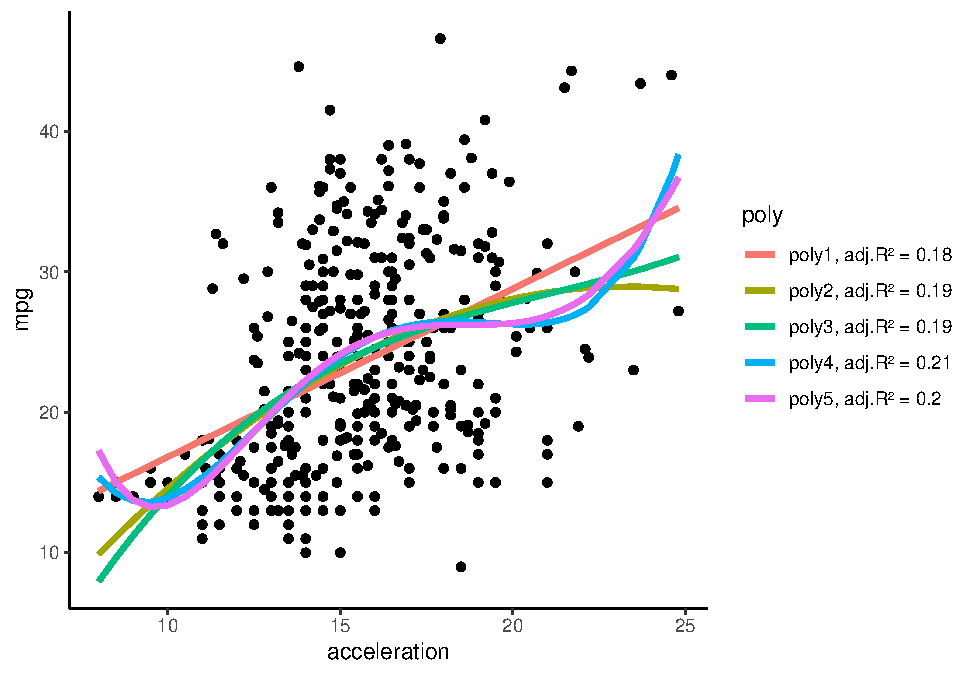
\includegraphics{leroy_francois_hw1_files/figure-latex/unnamed-chunk-4-1.pdf}

\newpage

\hypertarget{q2}{%
\chapter{Develop a model to predict whether a given car gets high or low gas mileage}\label{q2}}

\hypertarget{section-2}{%
\section{}\label{section-2}}

\textbf{Create a binary attribute, mpg01, that contains a 1 if mpg contains a value above its median,
and a 0 if mpg contains a value below its median. Create a single data set containing both mpg01 and the other Auto attributes except mpg. Compute entropy of mpg01.}

\begin{Shaded}
\begin{Highlighting}[]
\CommentTok{# Discretizing mpg}
\NormalTok{Auto}\OperatorTok{$}\NormalTok{mpg01 <-}\StringTok{ }\KeywordTok{ifelse}\NormalTok{(Auto}\OperatorTok{$}\NormalTok{mpg }\OperatorTok{>}\StringTok{ }\KeywordTok{median}\NormalTok{(Auto}\OperatorTok{$}\NormalTok{mpg), }\DecValTok{1}\NormalTok{, }\DecValTok{0}\NormalTok{)}
\CommentTok{# Creating dataset with discrete mpg}
\NormalTok{classif_data <-}\KeywordTok{subset}\NormalTok{(Auto, }\DataTypeTok{select =} \OperatorTok{-}\NormalTok{mpg)}
\CommentTok{## Compute entropy}
\CommentTok{# First compute the proba of each class}
\NormalTok{p <-}\StringTok{ }\KeywordTok{table}\NormalTok{(classif_data}\OperatorTok{$}\NormalTok{mpg01) }\OperatorTok{/}\StringTok{ }\KeywordTok{length}\NormalTok{(classif_data}\OperatorTok{$}\NormalTok{mpg01)}
\CommentTok{## Then compute the entropy}
\NormalTok{ent_mpg <-}\StringTok{ }\OperatorTok{-}\KeywordTok{sum}\NormalTok{(p }\OperatorTok{*}\StringTok{ }\KeywordTok{log2}\NormalTok{(p))}
\end{Highlighting}
\end{Shaded}

Here, the entropy of \(mpg01 =\) 1 which is totally expected because \texttt{mpg} has been discretized by its median, which means that \(50\%\) of \texttt{mpg} values are above (and thus equal to 1) and \(50\%\) are below (and thus equal to 0). Consequently, the probability of \texttt{mpg01} being 0 or 1 are both equal to \texttt{0.5} and the entropy is maximum.

\hypertarget{section-3}{%
\section{}\label{section-3}}

\textbf{Split the data into a training set and a test set 80:20}

\begin{Shaded}
\begin{Highlighting}[]
\KeywordTok{set.seed}\NormalTok{(}\DecValTok{123}\NormalTok{) }\CommentTok{# to reproduce the results}
\CommentTok{## Training dataset}
\NormalTok{train <-}\StringTok{ }\NormalTok{classif_data[}\KeywordTok{sample}\NormalTok{(}\KeywordTok{nrow}\NormalTok{(classif_data), }\KeywordTok{nrow}\NormalTok{(classif_data)}\OperatorTok{*}\FloatTok{0.8}\NormalTok{),]}
\CommentTok{## Test dataset}
\NormalTok{test <-}\StringTok{ }\NormalTok{classif_data[}\KeywordTok{sample}\NormalTok{(}\KeywordTok{nrow}\NormalTok{(classif_data), }\KeywordTok{nrow}\NormalTok{(classif_data)}\OperatorTok{*}\FloatTok{0.2}\NormalTok{),]}
\end{Highlighting}
\end{Shaded}

\hypertarget{section-4}{%
\section{}\label{section-4}}

\textbf{Make a trivial classifier (without using the features) and evaluate it on the test set. Compute its accuracy.}

\begin{Shaded}
\begin{Highlighting}[]
\CommentTok{# Most frequent class of the training data}
\KeywordTok{table}\NormalTok{(train}\OperatorTok{$}\NormalTok{mpg01)}
\end{Highlighting}
\end{Shaded}

\begin{verbatim}
## 
##   0   1 
## 154 159
\end{verbatim}

The most frequent class of the training dataset is \(1\). Thus, the trivial classifier will always predict \(1\).

\begin{Shaded}
\begin{Highlighting}[]
\CommentTok{## Confusion matrix of the trivial classifier}
\KeywordTok{table}\NormalTok{(test}\OperatorTok{$}\NormalTok{mpg01, }\KeywordTok{rep}\NormalTok{(}\DecValTok{1}\NormalTok{, }\KeywordTok{nrow}\NormalTok{(test)))}
\end{Highlighting}
\end{Shaded}

\begin{verbatim}
##    
##      1
##   0 42
##   1 36
\end{verbatim}

\begin{Shaded}
\begin{Highlighting}[]
\CommentTok{## Compute accuracy}
\NormalTok{accuracy <-}\StringTok{ }\DecValTok{36}\OperatorTok{/}\KeywordTok{nrow}\NormalTok{(test)}
\end{Highlighting}
\end{Shaded}

Here, the accuracy = 0.4615385, which means that only \(46\%\) of the target values will be classified correctly.

\newpage

\hypertarget{section-5}{%
\section{}\label{section-5}}

\textbf{Perform logistic regression on train in order to predict mpg01 using all the features except name. Use a threshold of 0.5 to cut the predicted probabilities to make class predictions.}

\hypertarget{compute-the-training-error-rate.}{%
\subsection{Compute the training error rate.}\label{compute-the-training-error-rate.}}

\begin{Shaded}
\begin{Highlighting}[]
\CommentTok{## Learn the model}
\NormalTok{logit_reg <-}\StringTok{ }\KeywordTok{glm}\NormalTok{(mpg01 }\OperatorTok{~}\StringTok{ }\NormalTok{., }\DataTypeTok{family =} \KeywordTok{binomial}\NormalTok{(}\DataTypeTok{link =} \StringTok{"logit"}\NormalTok{),}
                 \DataTypeTok{data =} \KeywordTok{subset}\NormalTok{(train, }\DataTypeTok{select =} \OperatorTok{-}\NormalTok{name))}
\CommentTok{## Use the model to predict on the learning dataset}
\NormalTok{train_prediction <-}\StringTok{ }\KeywordTok{predict}\NormalTok{(logit_reg, }\DataTypeTok{type =} \StringTok{"response"}\NormalTok{)}
\CommentTok{## Transform the prediction into 0/1}
\NormalTok{train_prediction <-}\StringTok{ }\KeywordTok{ifelse}\NormalTok{(train_prediction }\OperatorTok{>}\StringTok{ }\FloatTok{.5}\NormalTok{, }\DecValTok{1}\NormalTok{, }\DecValTok{0}\NormalTok{)}
\CommentTok{## Confusion matrix}
\NormalTok{cm_train_logit <-}\StringTok{ }\KeywordTok{table}\NormalTok{(train}\OperatorTok{$}\NormalTok{mpg01, train_prediction)}
\CommentTok{## Training error rate}
\NormalTok{train_error_rate <-}\StringTok{ }\DecValTok{1} \OperatorTok{-}\StringTok{ }\KeywordTok{sum}\NormalTok{(}\KeywordTok{diag}\NormalTok{(cm_train_logit))}\OperatorTok{/}\KeywordTok{sum}\NormalTok{(cm_train_logit)}
\end{Highlighting}
\end{Shaded}

The training error rate of this logistic regression is 0.0830671.

\newpage

\hypertarget{produce-a-confusion-matrix-comparing-the-true-test-target-values-to-the-predicted-test-target-values.-compute-the-test-error-rate-sensitivity-and-specificity.}{%
\subsection{Produce a confusion matrix comparing the true test target values to the predicted test target values. Compute the test error rate, Sensitivity, and Specificity.}\label{produce-a-confusion-matrix-comparing-the-true-test-target-values-to-the-predicted-test-target-values.-compute-the-test-error-rate-sensitivity-and-specificity.}}

\begin{Shaded}
\begin{Highlighting}[]
\CommentTok{## Use the model to predict on the test dataset}
\NormalTok{test_prediction <-}\StringTok{ }\KeywordTok{predict}\NormalTok{(logit_reg, }\DataTypeTok{type =} \StringTok{"response"}\NormalTok{, }\DataTypeTok{newdata =}\NormalTok{ test)}
\CommentTok{## Transform the prediction into 0/1}
\NormalTok{test_prediction <-}\StringTok{ }\KeywordTok{ifelse}\NormalTok{(test_prediction }\OperatorTok{>}\StringTok{ }\FloatTok{.5}\NormalTok{, }\DecValTok{1}\NormalTok{, }\DecValTok{0}\NormalTok{)}
\CommentTok{## Confusion matrix}
\NormalTok{cm_test_logit <-}\StringTok{ }\KeywordTok{table}\NormalTok{(test}\OperatorTok{$}\NormalTok{mpg01, test_prediction)}
\CommentTok{## Test error rate:}
\NormalTok{test_error_rate <-}\StringTok{ }\DecValTok{1} \OperatorTok{-}\StringTok{ }\KeywordTok{sum}\NormalTok{(}\KeywordTok{diag}\NormalTok{(cm_test_logit))}\OperatorTok{/}\KeywordTok{sum}\NormalTok{(cm_test_logit)}
\CommentTok{## Sensitivity}
\NormalTok{sensi <-}\StringTok{ }\NormalTok{cm_test_logit[}\DecValTok{2}\NormalTok{,}\DecValTok{2}\NormalTok{]}\OperatorTok{/}\NormalTok{(cm_test_logit[}\DecValTok{2}\NormalTok{,}\DecValTok{2}\NormalTok{] }\OperatorTok{+}\StringTok{ }\NormalTok{cm_test_logit[}\DecValTok{2}\NormalTok{,}\DecValTok{1}\NormalTok{])}
\CommentTok{## Specificity}
\NormalTok{speci <-}\StringTok{ }\NormalTok{cm_test_logit[}\DecValTok{1}\NormalTok{,}\DecValTok{1}\NormalTok{]}\OperatorTok{/}\NormalTok{(cm_test_logit[}\DecValTok{1}\NormalTok{,}\DecValTok{1}\NormalTok{]}\OperatorTok{+}\NormalTok{cm_test_logit[}\DecValTok{1}\NormalTok{,}\DecValTok{2}\NormalTok{])}
\end{Highlighting}
\end{Shaded}

The training error rate, sensitivity and specificity are respectively equal to 0.1153846, 0.9166667 and 0.8571429.

\hypertarget{provide-an-interpretation-of-each-hypothesis-parameter-in-the-model.}{%
\subsection{Provide an interpretation of each hypothesis parameter in the model.}\label{provide-an-interpretation-of-each-hypothesis-parameter-in-the-model.}}

The \textbf{test error rate} of 0.1153846 means that around 12\% of the predictions in both class are incorrect, \emph{i,e.} \(mpg = 1\) classified as \(0\) or \(mpg = 0\) classified as \(1\).

The \textbf{sensitivity} equal to 0.9166667 means that only 92\% of the example actually equal to 1 will correctly be classified as 1.

On the other hand, the \textbf{specificity} equal to 0.8571429 means that only 86\% of the examples equal to 0 will be corretly classified in the class 0.

\hypertarget{section-6}{%
\section{}\label{section-6}}

\textbf{In the previous exercise you used a threshold of 0.5. Re-run the experiment from the previous exercise with different threshold values, namely 0.1, 0.3, 0.6, 0.9.}

\begin{Shaded}
\begin{Highlighting}[]
\NormalTok{thresholds <-}\StringTok{ }\KeywordTok{c}\NormalTok{(}\FloatTok{0.1}\NormalTok{, }\FloatTok{0.3}\NormalTok{, }\FloatTok{0.5}\NormalTok{, }\FloatTok{0.6}\NormalTok{, }\FloatTok{0.9}\NormalTok{)}
\ControlFlowTok{for}\NormalTok{(i }\ControlFlowTok{in} \DecValTok{1}\OperatorTok{:}\KeywordTok{length}\NormalTok{(thresholds))\{}
  \CommentTok{## Use the model to predict on the test dataset}
\NormalTok{  test_prediction <-}\StringTok{ }\KeywordTok{predict}\NormalTok{(logit_reg, }\DataTypeTok{type =} \StringTok{"response"}\NormalTok{, }\DataTypeTok{newdata =}\NormalTok{ test)}
  \CommentTok{## Transform the prediction into 0/1}
\NormalTok{  test_prediction <-}\StringTok{ }\KeywordTok{ifelse}\NormalTok{(test_prediction }\OperatorTok{>}\StringTok{ }\NormalTok{thresholds[i], }\DecValTok{1}\NormalTok{, }\DecValTok{0}\NormalTok{)}
  \CommentTok{## Confusion matrix}
\NormalTok{  cm_test_logit <-}\StringTok{ }\KeywordTok{table}\NormalTok{(test}\OperatorTok{$}\NormalTok{mpg01, test_prediction)}
  \CommentTok{## Precision}
\NormalTok{  prec <-}\StringTok{ }\NormalTok{cm_test_logit[}\DecValTok{2}\NormalTok{,}\DecValTok{2}\NormalTok{]}\OperatorTok{/}\NormalTok{(cm_test_logit[}\DecValTok{2}\NormalTok{,}\DecValTok{2}\NormalTok{] }\OperatorTok{+}\StringTok{ }\NormalTok{cm_test_logit[}\DecValTok{1}\NormalTok{,}\DecValTok{2}\NormalTok{])}
  \CommentTok{## Recall}
\NormalTok{  recall <-}\StringTok{ }\NormalTok{cm_test_logit[}\DecValTok{2}\NormalTok{,}\DecValTok{2}\NormalTok{]}\OperatorTok{/}\NormalTok{(cm_test_logit[}\DecValTok{2}\NormalTok{,}\DecValTok{2}\NormalTok{] }\OperatorTok{+}\StringTok{ }\NormalTok{cm_test_logit[}\DecValTok{2}\NormalTok{,}\DecValTok{1}\NormalTok{])}
  \CommentTok{## F-measure}
\NormalTok{  fmeasure <-}\StringTok{ }\DecValTok{2}\OperatorTok{*}\NormalTok{(prec}\OperatorTok{*}\NormalTok{recall)}\OperatorTok{/}\NormalTok{(prec}\OperatorTok{+}\NormalTok{recall)}
  \CommentTok{#Print}
  \KeywordTok{cat}\NormalTok{(}\KeywordTok{paste0}\NormalTok{(}\StringTok{"-"}\NormalTok{,}\StringTok{" For threshold = "}\NormalTok{, thresholds[i],}
               \StringTok{" , Precision = "}\NormalTok{, prec,}
               \StringTok{" , Recall = "}\NormalTok{, recall,}
               \StringTok{" and F-measure = "}\NormalTok{, fmeasure), }\DataTypeTok{sep =} \StringTok{"}\CharTok{\textbackslash{}n}\StringTok{"}\NormalTok{)}
\NormalTok{\}}
\end{Highlighting}
\end{Shaded}

\begin{itemize}
\tightlist
\item
  For threshold = 0.1 , Precision = 0.765957446808511 , Recall = 1 and F-measure = 0.867469879518072
\item
  For threshold = 0.3 , Precision = 0.772727272727273 , Recall = 0.944444444444444 and F-measure = 0.85
\item
  For threshold = 0.5 , Precision = 0.846153846153846 , Recall = 0.916666666666667 and F-measure = 0.88
\item
  For threshold = 0.6 , Precision = 0.833333333333333 , Recall = 0.833333333333333 and F-measure = 0.833333333333333
\item
  For threshold = 0.9 , Precision = 0.961538461538462 , Recall = 0.694444444444444 and F-measure = 0.806451612903226
\end{itemize}

We can see the that recall (\emph{i.e.} precision) is decreasing with the increasing threshold. It means that with a low threshold and a high recall, most of the mpg = 1 will be correctly classified into class 1. For instance, for threshold = 0.1, recall = 1, which means that all the actual mpg = 1 are classified as 1.

On the other hand, we can see that the the precision has the opposite behavior to the recall: the precision increases with the increasing threshold. A higher precision means that the predicted class = 1 will contain mostly actual values of mpg = 1 and will contain less misclassifications.

We can see that the F-score, which takes into account both precision and recall, is the highest for threshold = 0.5. Thus, it seems that we should prefer this threshold of 0.5 over the others because it optimizes the recall and precision metrics.

\newpage

\hypertarget{section-7}{%
\section{}\label{section-7}}

\textbf{Perform decision tree algorithm on train to predict mpg01 using all the features except name.}

\hypertarget{create-a-plot-of-the-tree.-compute-the-training-error-rate.-compute-the-test-error-rate.}{%
\subsection{Create a plot of the tree. Compute the training error rate. Compute the test error rate.}\label{create-a-plot-of-the-tree.-compute-the-training-error-rate.-compute-the-test-error-rate.}}

\begin{Shaded}
\begin{Highlighting}[]
\CommentTok{## Learn the decision tree}
\NormalTok{dt <-}\StringTok{ }\KeywordTok{rpart}\NormalTok{(}\KeywordTok{as.factor}\NormalTok{(mpg01) }\OperatorTok{~}\StringTok{ }\NormalTok{., }\DataTypeTok{data =} \KeywordTok{subset}\NormalTok{(train, }\DataTypeTok{select =} \OperatorTok{-}\NormalTok{name))}
\CommentTok{## Plot it}
\KeywordTok{rpart.plot}\NormalTok{(dt)}
\end{Highlighting}
\end{Shaded}

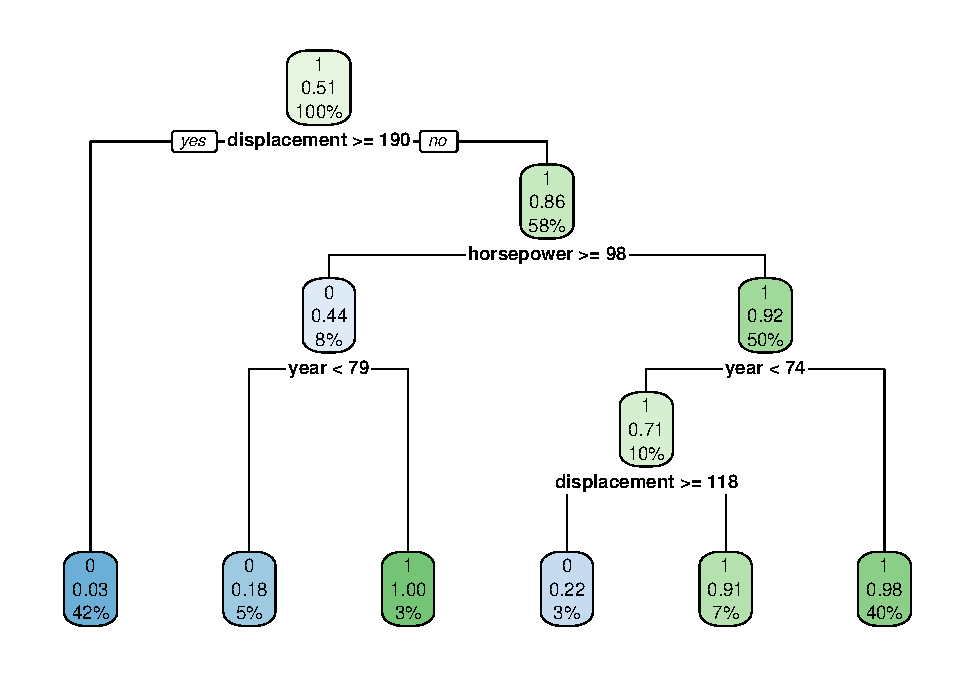
\includegraphics{leroy_francois_hw1_files/figure-latex/unnamed-chunk-14-1.pdf}

\begin{Shaded}
\begin{Highlighting}[]
\CommentTok{## Training data}
\NormalTok{predtrain <-}\StringTok{ }\KeywordTok{predict}\NormalTok{(dt, }\DataTypeTok{type =} \StringTok{"class"}\NormalTok{)}
\NormalTok{cmtrain <-}\StringTok{ }\KeywordTok{table}\NormalTok{(train}\OperatorTok{$}\NormalTok{mpg01, predtrain)}
\NormalTok{trainerrorrate <-}\StringTok{ }\DecValTok{1} \OperatorTok{-}\StringTok{ }\NormalTok{(}\KeywordTok{sum}\NormalTok{(}\KeywordTok{diag}\NormalTok{(cmtrain))}\OperatorTok{/}\KeywordTok{sum}\NormalTok{(cmtrain))}
\CommentTok{## Test data}
\NormalTok{predtest <-}\StringTok{ }\KeywordTok{predict}\NormalTok{(dt, }\DataTypeTok{type =} \StringTok{"class"}\NormalTok{, }\DataTypeTok{newdata =}\NormalTok{ test)}
\NormalTok{cmtest <-}\StringTok{ }\KeywordTok{table}\NormalTok{(test}\OperatorTok{$}\NormalTok{mpg01, predtest)}
\NormalTok{testerrorrate <-}\StringTok{ }\DecValTok{1} \OperatorTok{-}\StringTok{ }\NormalTok{(}\KeywordTok{sum}\NormalTok{(}\KeywordTok{diag}\NormalTok{(cmtest))}\OperatorTok{/}\KeywordTok{sum}\NormalTok{(cmtest))}
\end{Highlighting}
\end{Shaded}

The training error rate = 0.0447284 and the test error rate = 0.1025641.

\hypertarget{tune-the-cp-parameter.-choose-the-best-value-of-cp-and-evaluate-your-model-again.-what-is-the-best-value-of-cp-why-explain-it-explicitly.-compute-the-accuracy-of-the-model-with-your-best-cp.}{%
\subsection{Tune the cp parameter. Choose the best value of cp, and evaluate your model again. What is the best value of cp? Why? Explain it explicitly. Compute the accuracy of the model with your best cp.}\label{tune-the-cp-parameter.-choose-the-best-value-of-cp-and-evaluate-your-model-again.-what-is-the-best-value-of-cp-why-explain-it-explicitly.-compute-the-accuracy-of-the-model-with-your-best-cp.}}

\begin{Shaded}
\begin{Highlighting}[]
\NormalTok{tunedDT <-}\StringTok{ }\KeywordTok{rpart}\NormalTok{(}\KeywordTok{as.factor}\NormalTok{(mpg01) }\OperatorTok{~}\StringTok{ }\NormalTok{., }\DataTypeTok{data =} \KeywordTok{subset}\NormalTok{(train, }\DataTypeTok{select =} \OperatorTok{-}\NormalTok{name), }
                 \DataTypeTok{cp =} \FloatTok{0.004}\NormalTok{)}
\KeywordTok{plotcp}\NormalTok{(tunedDT)}
\end{Highlighting}
\end{Shaded}

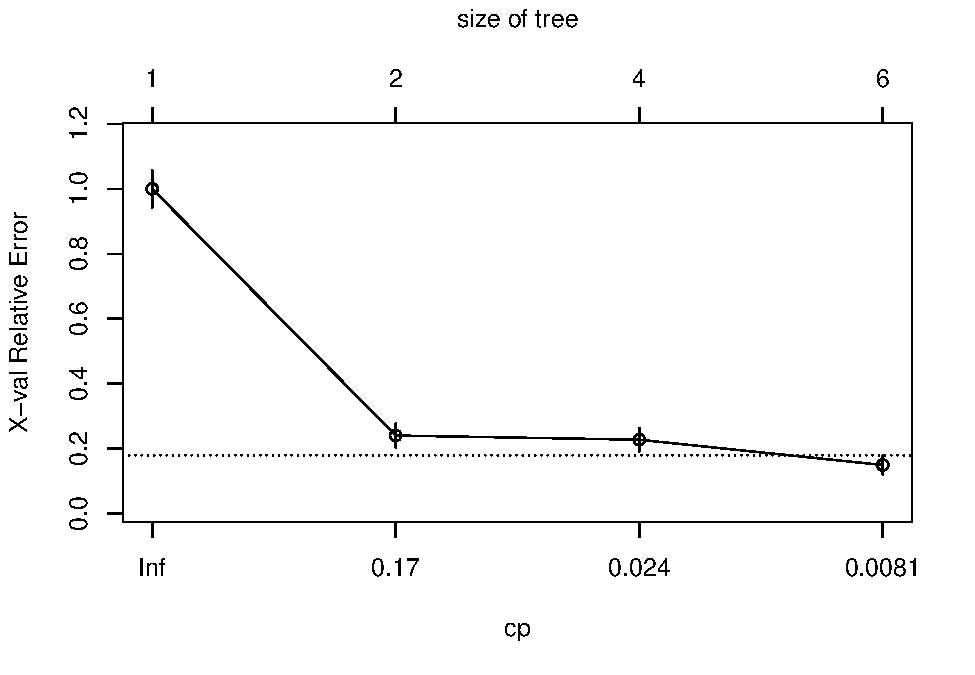
\includegraphics{leroy_francois_hw1_files/figure-latex/unnamed-chunk-15-1.pdf}

\begin{tabular}{r|r|r|r|r}
\hline
CP & nsplit & rel error & xerror & xstd\\
\hline
0.8051948 & 0 & 1.0000000 & 1.0000000 & 0.0574336\\
\hline
0.0357143 & 1 & 0.1948052 & 0.2402597 & 0.0370905\\
\hline
0.0162338 & 3 & 0.1233766 & 0.2272727 & 0.0362046\\
\hline
0.0040000 & 5 & 0.0909091 & 0.1493506 & 0.0299757\\
\hline
\end{tabular}

The most optimal value of cp (\emph{i.e.} complexity parameter) is the one minimizing the \texttt{xerror}, which is the generalization error (\emph{i.e.} true error or expected error) that estimates the probability of error on an other potential dataset of distribution \(D\).

The accuracy of the new decision tree is 0.8974359.

\newpage

\hypertarget{section-8}{%
\section{}\label{section-8}}

\textbf{Compare the best models trained in the previous exercises 4., 5., and 6. Which one could be considered as the best?}

\begin{longtable}[]{@{}ll@{}}
\toprule
Method & Error rate\tabularnewline
\midrule
\endhead
Logistic Regression & 0.1153846\tabularnewline
Decision Tree & 0.1025641\tabularnewline
\bottomrule
\end{longtable}

Using the test error rate as the final metric to choose the best modeling method, it seems that the decision tree has a slightly lower error rate and should be considered the best.


\singlespacing % reset the spacing of the bibliography style
\end{document}
